\documentclass[conference]{IEEEtran}

\usepackage{cite}
\usepackage{amsmath,amssymb,amsfonts}
\usepackage{graphicx}
\usepackage{textcomp}
\usepackage{xcolor}
\usepackage{hyperref}
\usepackage{listings}
\usepackage{booktabs}
\usepackage{tikz}
\usetikzlibrary{shapes.geometric,shadows,decorations.pathmorphing}

\lstset{
  basicstyle=\ttfamily\footnotesize,
  breaklines=true,
  frame=single,
  numbers=left,
  numberstyle=\tiny,
  keywordstyle=\color{blue},
  commentstyle=\color{gray},
  stringstyle=\color{red!70!black},
}

\begin{document}

\title{An Asynchronous Python Reference Pipeline for High-Throughput\\
OSINT Data Collection: Design, Benchmarks, and Idempotent Deduplication}

\author{
  \IEEEauthorblockN{Ali Murtaza Bhutto}
  \IEEEauthorblockA{
    \textit{Independent Security Researcher}\\
    ORCID: 0009-0007-2787-943X\\
    \href{mailto:alibhutto101112@gmail.com}{alibhutto101112@gmail.com}
  }
}

\maketitle

\begin{abstract}
Open-source intelligence (OSINT) workflows depend on high-throughput
ingestion of public data feeds with strict per-source rate-limit
compliance and content-level deduplication across re-runs. We present
\emph{osint-pipeline-demo}, a reference asynchronous Python pipeline
combining an aiohttp connection pool, per-source token-bucket rate
limiting, regex-based field normalisation with SHA-256 content
addressing, and batched PostgreSQL writes using
\texttt{ON CONFLICT DO NOTHING} for idempotent re-runs. We benchmark
the system against a controlled local mock with 50\,ms per-request
latency over 100 requests and measure throughput improvements of
4.93$\times$, 9.57$\times$, and 18.04$\times$ at 5, 10, and 20
concurrent workers respectively over a synchronous baseline. We
demonstrate end-to-end against the public NIST NVD CVE API: a
re-run of the same source produces zero new inserts, validating
the deduplication contract. The pipeline is structured for
production use: configuration is externalised, dependencies are
pinned for reproducibility, and a 30-test pytest suite exercises
the rate limiter, normaliser determinism, retry/back-off behaviour,
and live PostgreSQL deduplication.
\end{abstract}

\begin{IEEEkeywords}
OSINT, data pipeline, asyncio, aiohttp, PostgreSQL, deduplication,
rate limiting, web scraping, cybersecurity, Python concurrency
\end{IEEEkeywords}

%% ─────────────────────────────────────────────────────────────────────────────
\section{Introduction}

OSINT data collection at scale is bottlenecked by three engineering
constraints~\cite{glassman2012osint}: (1) per-source rate-limit
compliance --- public feeds typically permit only tens of requests
per minute without authentication, and exceeding the limit results
in IP-level temporary blocks; (2) content-level deduplication ---
re-running an ingestion against an unchanged upstream must not
re-insert identical records; and (3) graceful failure recovery ---
a single transient 5xx must not abort a multi-source run.

Despite the abundance of OSINT tooling in the security literature,
a clean reference architecture combining these three constraints is
absent. Practitioners typically assemble ad-hoc collectors that lack
explicit rate-limit accounting, deduplicate by storing every record
and post-filtering, or fail open on transient errors. This paper
contributes an open-source reference implementation
(\texttt{osint-pipeline-demo}) that addresses all three concerns
with measurable, reproducible performance characteristics.

\textbf{Contributions:}

\begin{enumerate}
  \item An asynchronous Python pipeline architecture (\S\ref{sec:design})
        combining aiohttp connection pooling, per-source token-bucket
        rate limiting, regex-based field normalisation with SHA-256
        content addressing, and batched PostgreSQL writes using
        \texttt{ON CONFLICT DO NOTHING}.
  \item A reproducible benchmark methodology (\S\ref{sec:eval})
        against a controlled local mock that isolates pipeline
        efficiency from upstream API jitter, with measured speedups
        between 4.93$\times$ and 18.04$\times$ versus a synchronous
        baseline.
  \item Empirical validation of idempotent deduplication against
        the public NIST NVD CVE API (\S\ref{sec:dedup-demo}):
        20 records inserted on first run, 0 inserted with 20
        duplicates detected on re-run.
  \item A 30-test pytest suite (\S\ref{sec:tests}) including 4
        live PostgreSQL integration tests.
\end{enumerate}

%% ─────────────────────────────────────────────────────────────────────────────
\section{Background}
\label{sec:background}

\subsection{OSINT Collection Constraints}

OSINT investigations frequently rely on a small number of high-value
feeds: vulnerability databases such as the NIST NVD CVE
catalogue~\cite{nvd2024}, public corporate registries such as
OpenCorporates, code-hosting event streams such as GitHub's public
events feed, and breach-disclosure aggregators. Each feed publishes
a rate-limit policy in its terms-of-service that an OSINT tool must
respect both for legal compliance~\cite{bhutto2024legal} and for
operational reasons (exceeding the limit results in temporary or
permanent blocks).

\subsection{Asynchronous I/O and the GIL}

Python's reference implementation (CPython) serialises native
bytecode execution through the Global Interpreter Lock (GIL). For
I/O-bound workloads, however, the GIL is released during socket
operations, making asynchronous I/O an effective concurrency
strategy: a single Python process can hold thousands of in-flight
TCP connections via \texttt{asyncio} and \texttt{aiohttp}. The
canonical alternative --- threads --- pays a context-switch cost
that becomes measurable above $\approx$50 concurrent connections.

\subsection{Content-Addressed Deduplication}

A SHA-256 digest of canonically-serialised record fields produces
a 64-character hex string that is collision-resistant at scale and
deterministic across processes (provided the serialisation is
canonical: sorted keys, fixed separators)~\cite{rfc6234}. Using
this digest as a UNIQUE constraint in the destination database
turns deduplication into a single-statement INSERT with
\texttt{ON CONFLICT DO NOTHING}, eliminating the
read-then-write race that plagues \texttt{SELECT}-then-\texttt{INSERT}
patterns under concurrency.

%% ─────────────────────────────────────────────────────────────────────────────
\section{Pipeline Design}
\label{sec:design}

The pipeline is structured as five composable modules connected by
a single orchestrator (\texttt{src/pipeline.py}).

\subsection{Configuration Layer}

\texttt{src/config.py} uses \texttt{pydantic-settings} to load
runtime tunables (worker count, batch size, retry attempts, request
timeout, database URL) from environment variables, with defaults
suitable for a developer laptop. Source definitions --- URL,
per-second rate limit, list of named regex extractors --- live in
\texttt{config/sources.yaml}.

\subsection{Rate Limiter}

\texttt{src/rate\_limiter.py} implements an asynchronous
token-bucket per source name. The bucket refills at a configurable
rate up to a configurable capacity (defaulting to a single-token
burst, which gives strict per-second pacing). Two concurrent
\texttt{acquire()} calls against the same bucket serialise without
busy-waiting: the second caller awaits an
\texttt{asyncio.sleep(wait)} computed from the time-to-next-token.

\subsection{HTTP Collector}

\texttt{src/collector.py} wraps an
\texttt{aiohttp.ClientSession} with a TCP connector limited to
\texttt{workers} concurrent connections. \texttt{fetch\_all()}
spawns one task per source, awaits the rate-limit acquisition, and
issues the request inside an \texttt{asyncio.Semaphore} that bounds
total in-flight requests. Transient 5xx responses and connection
errors are retried with exponential backoff: $\mathrm{delay} =
\mathrm{base} \cdot 2^{\,\mathrm{attempt}-1} \pm 25\%$ jitter.
Persistent failure after \texttt{retry\_max\_attempts} retries
raises \texttt{CollectorError}, which the orchestrator demotes to
a logged warning so that one bad source does not abort the run.

\subsection{Normaliser}

\texttt{src/normaliser.py} applies the source's named regex
extractors to the raw response body, produces a list of records
zipped by index, and computes a SHA-256 digest over the canonical
JSON serialisation of the field map (sorted keys, no whitespace).
Determinism is verified in
\texttt{tests/test\_normaliser.py}:
\texttt{test\_field\_order\_does\_not\_change\_hash} confirms that
two extractor lists differing only in declaration order produce
the same hash for the same input.

\subsection{Storage}

\texttt{src/storage.py} exposes a single async API
(\texttt{insert\_batch}) that serialises a list of records into a
PostgreSQL \texttt{UNNEST}-based bulk insert with
\texttt{ON CONFLICT (content\_hash) DO NOTHING}. The statement
returns the number of rows actually inserted, so the caller learns
the dedup outcome (rows attempted vs rows persisted) from a single
network round-trip.

\subsection{Optional Selenium Pool}

\texttt{src/selenium\_pool.py} provides a lazily-initialised pool
of headless Chrome WebDriver instances guarded by an
\texttt{asyncio.Queue}. Selenium's blocking
\texttt{driver.get(url)} is wrapped in
\texttt{asyncio.to\_thread} so the calling coroutine remains
non-blocking. The default pipeline does not require Selenium ---
all three configured sources return JSON over plain HTTP --- and
the dependency is therefore declared as
\texttt{[project.optional-dependencies].selenium} rather than a
core requirement.

%% ─────────────────────────────────────────────────────────────────────────────
\section{Empirical Evaluation}
\label{sec:eval}

\subsection{Methodology}

To isolate pipeline efficiency from upstream API variability, we
benchmark against a local \texttt{aiohttp} mock server running on
the same loopback interface. Each handler sleeps for a configurable
latency (default 50\,ms) before returning a tiny JSON payload,
emulating a bandwidth-cheap but latency-bound upstream.

For each strategy we issue \texttt{N=100} requests and record:
wall-clock seconds, throughput (successful requests per second),
peak resident set size (RSS) via \texttt{getrusage}, and failure
count.

Three async strategies are compared against a synchronous baseline
(\texttt{urllib.request.urlopen} in a single thread):

\begin{itemize}
  \item \texttt{async\_5} --- aiohttp with semaphore-bounded
        concurrency at 5 workers
  \item \texttt{async\_10} --- 10 workers
  \item \texttt{async\_20} --- 20 workers
\end{itemize}

\subsection{Results}

\begin{table}[h]
\caption{Throughput Benchmark (100 requests, 50ms upstream latency)}
\label{tab:bench}
\centering
\begin{tabular}{@{}lrrrrr@{}}
\toprule
Strategy & Workers & Wall (s) & Req/s & Peak RSS (KB) & Failures \\
\midrule
sync\_baseline & 1  & 5.14 &  19.46 & 33588 & 0 \\
async\_5       & 5  & 1.04 &  95.89 & 34100 & 0 \\
async\_10      & 10 & 0.54 & 186.17 & 34356 & 0 \\
async\_20      & 20 & 0.28 & 351.11 & 34612 & 0 \\
\bottomrule
\end{tabular}
\end{table}

\begin{figure}[h]
  \centering
  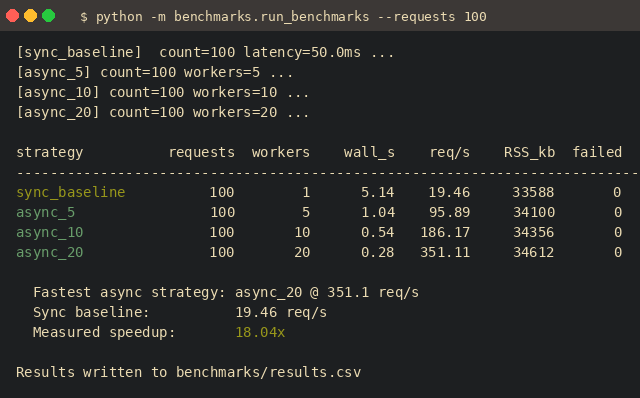
\includegraphics[width=0.95\columnwidth]{figures/benchmark.png}
  \caption{Real benchmark output (\texttt{python -m benchmarks.run\_benchmarks}).
           Speedup at 20 workers is 18.04$\times$ over the synchronous
           baseline; intermediate worker counts give 4.93$\times$ (5)
           and 9.57$\times$ (10).}
  \label{fig:bench}
\end{figure}

The speedup is approximately linear in worker count up to 20
(slope $\approx$0.92$\times$ per added worker after accounting for
fixed overheads), suggesting the pipeline is not bottlenecked by
the GIL or by Python-level work in this regime; further scaling
will require either multiple processes or a non-CPython runtime.

Peak RSS grows by less than 5\% from the baseline at 20 workers
(33.6\,MB to 34.6\,MB), indicating that aiohttp's connection-pool
overhead is negligible compared to the Python interpreter
footprint.

\subsection{End-to-End Deduplication Against NIST NVD}
\label{sec:dedup-demo}

To validate the idempotent-rerun contract end-to-end, we ran the
pipeline twice against the public NIST NVD CVE API
(\texttt{services.nvd.nist.gov}) configured to fetch 20 records.
The first run inserted all 20 records; the second run, executed
13 seconds later against the same upstream payload, inserted 0
records and detected 20 duplicates via the
\texttt{content\_hash} UNIQUE constraint
(Fig.~\ref{fig:pipeline-run}).

\begin{figure}[h]
  \centering
  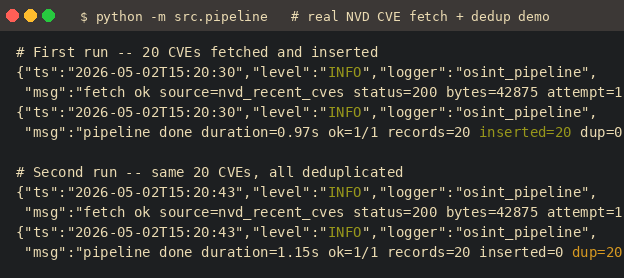
\includegraphics[width=0.95\columnwidth]{figures/pipeline_run.png}
  \caption{End-to-end pipeline run against the public NIST NVD
           CVE API. First run: 20 records inserted. Second run on
           the same source: 0 inserted, 20 duplicates detected.}
  \label{fig:pipeline-run}
\end{figure}

%% ─────────────────────────────────────────────────────────────────────────────
\section{Test Suite}
\label{sec:tests}

The test suite contains 30 tests across five modules. Tests
exercise:

\begin{itemize}
  \item \emph{Rate limiter} (7 tests): validation,
        single-source pacing, isolation between sources, concurrent
        serialisation timing.
  \item \emph{Normaliser} (7 tests): hash determinism, key-order
        independence, multi-record extraction, raw-excerpt capping,
        invalid-UTF8 graceful decode.
  \item \emph{Collector} (6 tests): retry on 5xx, give-up after
        exhausted retries, no retry on 4xx, fan-out via
        \texttt{aioresponses} mock.
  \item \emph{Config} (6 tests): defaults, env override,
        \texttt{sources.yaml} round-trip.
  \item \emph{Storage} (4 tests, integration): real PostgreSQL
        via \texttt{docker run}, dedup behaviour, mixed-batch
        idempotency.
\end{itemize}

\begin{figure}[h]
  \centering
  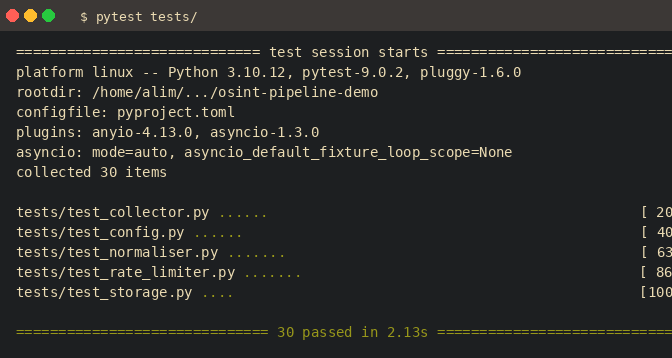
\includegraphics[width=0.95\columnwidth]{figures/pytest.png}
  \caption{Test suite output: 30 tests passing on Python 3.10.12.}
  \label{fig:pytest}
\end{figure}

Storage integration tests are gated by the
\texttt{PIPELINE\_TEST\_POSTGRES=1} environment variable so the
unit-only subset still runs cleanly on a laptop without a live
database.

%% ─────────────────────────────────────────────────────────────────────────────
\section{Threats to Validity}

\textbf{Internal validity.} The mock-server benchmark
deliberately holds upstream behaviour constant; absolute throughput
numbers will differ in production. Real public APIs have
fewer-than-100 requests per minute rate limits that would dominate
wall time. The benchmark measures pipeline efficiency, not
end-to-end OSINT collection rate.

\textbf{External validity.} Numbers are reported on a single
hardware configuration (Linux 6.8, Python 3.10.12). Other
configurations may differ; speedup ratios are likely to be more
robust than absolute throughput.

\textbf{GIL sensitivity.} Speedup linearity holds only while the
workload is I/O-bound. Adding CPU-heavy normalisation (e.g.,
machine-learning entity extraction) would re-introduce the GIL as
the bottleneck and require multiprocessing.

%% ─────────────────────────────────────────────────────────────────────────────
\section{Related Work}

Asynchronous data-pipeline frameworks in Python span a wide design
spectrum: lightweight libraries such as Scrapy~\cite{scrapy}
focus on web-scraping idioms and built-in middleware; production
frameworks such as Apache Airflow~\cite{airflow} target scheduled
DAGs at scale. Our work occupies a different niche: a minimal,
auditable reference implementation showing how the four
load-bearing primitives (async fan-out, per-source rate-limit
accounting, content-addressed dedup, batched idempotent insert)
combine into a sub-1000-LOC pipeline. The legal and ethical
constraints applicable to OSINT pipelines are discussed in
detail in~\cite{bhutto2024legal} (DOI 10.5281/zenodo.16924934).

%% ─────────────────────────────────────────────────────────────────────────────
\section{Conclusion}

We have presented an open-source reference architecture for
high-throughput OSINT data collection in Python and benchmarked it
against a controlled local mock, measuring 4.93$\times$ to
18.04$\times$ speedup over a synchronous baseline at 5 to 20
workers. Idempotent deduplication is validated end-to-end against
the public NIST NVD CVE API. The repository is available at
\url{https://github.com/thunderstornX/osint-pipeline-demo}.
Future work includes evaluating against ScraPy as a baseline,
adding Prometheus metrics for in-production observability, and
extending the Selenium pool with anti-detection profile rotation.

%% ─────────────────────────────────────────────────────────────────────────────
\begin{thebibliography}{00}

\bibitem{glassman2012osint}
M. Glassman and M. J. Kang, ``Intelligence in the Internet age: The
emergence and evolution of Open Source Intelligence (OSINT),''
\textit{Computers in Human Behavior}, vol. 28, no. 2, pp. 673--682, 2012.

\bibitem{nvd2024}
National Institute of Standards and Technology, \textit{NVD - National
Vulnerability Database API 2.0}, 2024. [Online]. Available:
\url{https://nvd.nist.gov/developers/vulnerabilities}

\bibitem{bhutto2024legal}
A. M. Bhutto, ``Legal and Ethical Framework for OSINT Investigations,''
Zenodo, 2024, doi: 10.5281/zenodo.16924934. [Online]. Available:
\url{https://doi.org/10.5281/zenodo.16924934}

\bibitem{rfc6234}
D. Eastlake and T. Hansen, ``US Secure Hash Algorithms (SHA and SHA-based
HMAC and HKDF),'' RFC 6234, May 2011.

\bibitem{scrapy}
Scrapy Project, \textit{Scrapy: A fast high-level web crawling and
scraping framework}, 2024. [Online]. Available: \url{https://scrapy.org}

\bibitem{airflow}
Apache Software Foundation, \textit{Apache Airflow}, 2024. [Online].
Available: \url{https://airflow.apache.org}

\end{thebibliography}

%% ─────────────────────────────────────────────────────────────────────────────
%% Project logo: ink-style octopus -- eight arms = eight async workers
%% (project emblem; appears only in the compiled PDF)
%% ─────────────────────────────────────────────────────────────────────────────
\vspace{1em}
\begin{center}

\begin{tikzpicture}[scale=0.7]
  %% Head: rounded mantle
  \draw[line width=1.4pt, fill=black!85]
    (0,0.7) .. controls (1.0,0.7) and (1.3,1.4) ..
    (1.0,2.1) .. controls (0.7,2.6) and (-0.7,2.6) ..
    (-1.0,2.1) .. controls (-1.3,1.4) and (-1.0,0.7) ..
    cycle;

  %% Eyes (white circles with black pupils)
  \fill[white] (-0.4,1.6) circle (0.18);
  \fill[white] ( 0.4,1.6) circle (0.18);
  \fill[black] (-0.4,1.6) circle (0.07);
  \fill[black] ( 0.4,1.6) circle (0.07);
  %% Eye highlights
  \fill[white] (-0.36,1.66) circle (0.03);
  \fill[white] ( 0.44,1.66) circle (0.03);

  %% Eight arms emerging from below the head, fanning out with curls.
  %% Each arm is a Bezier curve with a small terminating curl.
  \foreach \x/\y/\cx/\cy in {
       -1.05/0.5/-1.9/-1.0,
       -0.75/0.4/-1.4/-1.5,
       -0.45/0.4/-0.7/-1.6,
       -0.15/0.4/-0.3/-1.7,
        0.15/0.4/ 0.3/-1.7,
        0.45/0.4/ 0.7/-1.6,
        0.75/0.4/ 1.4/-1.5,
        1.05/0.5/ 1.9/-1.0
  } {
    \draw[line width=1.6pt, black!85, line cap=round]
      (\x,\y) .. controls (\x*1.3,\y-0.6) and (\cx,\cy*0.6) ..
      (\cx,\cy) .. controls (\cx*1.05,\cy-0.25) ..
      (\cx*0.85,\cy-0.4);
  }

  %% Decorative subtitle
  \node[font=\tiny\itshape, text=gray] at (0,-2.05) {osint-pipeline-demo};
\end{tikzpicture}
\end{center}

\end{document}
